%%%%%%%%%%%%%%%%%%%%%%%%%%%%%%%%%%%%%%%%%%%%%%%%%%%%%%%%
% Este é um documento que servirá de modelo para
% os relatórios feitos na disciplina Circuitos Digitais
% 2016-2
%%%%%%%%%%%%%%%%%%%%%%%%%%%%%%%%%%%%%%%%%%%%%%%%%%%%%%%%%

\PassOptionsToPackage{brazil,american}{babel}
\documentclass[12pt]{article}

\usepackage{sbc-template}
\usepackage[brazil,american]{babel}
\usepackage[utf8]{inputenc}

\usepackage{graphicx}
\usepackage{url}
\usepackage{float}
\usepackage{listings}
\usepackage{color}
\usepackage{todonotes}
\usepackage{algorithmic}
\usepackage{algorithm}
\usepackage{hyperref}
     
\sloppy

\title{Experimento 6\\ 
	Circuitos Combinacionais: Codificador e Decodificador}

\author{
	Lucas Mafra Chagas, 12/0126443 \\
	Marcelo Giordano Martins Costa de Oliveira,  12/0037301
}


\address{Dep. Ciência da Computação -- Universidade de Brasília (UnB)\\
	CiC 116351 - Circuistos Digitais - Turma C
	\email{\{giordano.marcelo, chagas.lucas.mafra\}@gmail.com}
}

\begin{document} 

\maketitle

 \begin{abstract}
   In this experiment, we buit a coder and a decoder using the Quartus II software.
 \end{abstract}
     
 \begin{resumo} 
	Nesse experimento, implementamos um codificador e um decodificador usando o software Quartus II.
 \end{resumo}


\section{Objetivos}
\label{sec:Objetivos}

Elaboração de um codificador e de um decodificador usando-se circuitos combinacionais e
aplicando-se as técnicas de minimização de funções lógicas. Verificação da possibilidade
de conversão de um número decimal em um número binário de código qualquer e sua
posterior decodificação.

\section{Materiais} 
\label{sec:Materiais}

\begin{itemize}
    \item Software Quartus II versão 13.0
	\item Kit de desenvolvimento em FPGA DE2 Altera
    
\end{itemize}


\section{Introdução}
\label{sec:Introducao}

Os computadores são máquinas que trabalham com a utilização de um sistema binário para analisar variáveis e realizar cálculos. Já o homem está acostumado a raciocinar e trabalhar com o sistema decimal. Portanto, para que a comunicação homem-máquina possa ser feita de maneira mais direta, sem que o homem precise aprender a interpretar números binários, convém incorporar aos equipamentos de entrada e saída de computadores conversores de código decimal-binário e binário-decimal, respectivamente. Para o primeiro caso(onde a entrada é um número decimal), temos que o conversor é chamado de codificador, enquanto para o segundo caso (onde a saída é um número decimal) ele é chamado de decodificador.

\begin{figure}[H]
	\centering
	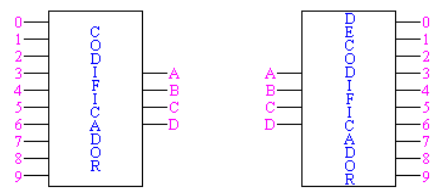
\includegraphics[width=.5\textwidth]{coddecod.jpg}
	\caption{Codificador e Decodificador.}
	\label{fig:coddecod}
\end{figure}


Para o codificador, teremos uma, e somente uma, entrada ativada a cada instante. A saída corresponderá à forma codificada desse decimal (utilizando apenas 0’s e 1’s). Já para o decodificador, temos que todas as entradas são ativadas no mesmo instante, porém, elas geram apenas uma saída. 
Para este experimento, será criado um codificafor decimal-Código de Gray e um decodificador Código de Gray-binário. Este código é determinado como apresenta a tabela abaixo:

\begin{table}[H]
	\centering
	\begin{tabular}{|c|c|c|c|c|}
		\cline{1-5}
		\multicolumn{1}{|c|}{Decimal} & \multicolumn{1}{|c|}{A} & \multicolumn{1}{|c|}{B} & \multicolumn{1}{|c|}{C} & \multicolumn{1}{|c|}{D}\\
		\hline
		0 & 0 & 0 & 0 & 0 \\
		\hline
		1 & 0 & 0 & 0 & 1 \\
		\hline
		2 & 0 & 0 & 1 & 1 \\
		\hline
		3 & 0 & 0 & 1 & 0 \\
		\hline
		4 & 0 & 1 & 1 & 0 \\
		\hline
		5 & 0 & 1 & 1 & 1 \\
		\hline
		6 & 0 & 1 & 0 & 1 \\
		\hline
		7 & 0 & 1 & 0 & 0 \\
		\hline
		8 & 1 & 1 & 0 & 0 \\
		\hline
		9 & 1 & 1 & 0 & 1 \\
		\hline
	\end{tabular}
	
\end{table} 




\section{Procedimentos}
\label{sec:Procedimentos}

Neste relatório, precisamos fazer:
\begin{itemize}
	\item Obter as funções booleanas para o codificador.
	\item Fazer simulações funcional e temporal do diagrama lógico do codificador no Quartus. 
	\item Obter as funções booleanas para o decodificador.
	\item Fazer simulações funcional e temporal do diagrama lógico do decodificador no Quartus. 
	\item Filmar o funcionamento do codificador e decodificador feito no Quartus II.
\end{itemize}

\subsection{Funções Booleanas para o Codificador}
\label{sec:Cod}

É possível obter as seguintes funções booleanas para o codificador utilizando o mapa de Karnaugh:

$A = (8+9) = \overline{\overline{8}.\overline{9}}$

$B = (4 + 5 + 6 + 7 + 8 + 9) = \overline{\overline{4}.\overline{5}.\overline{6}.\overline{7}.\overline{8}.\overline{9}} $

$C = (2 + 3 + 4 + 5) = \overline{\overline{2}.\overline{3}.\overline{4}.\overline{5}}$

$D = (1 + 2 + 5 + 6 + 9) = \overline{\overline{1}.\overline{2}.\overline{5}.\overline{6}.\overline{9}}$

Com as fórmulas supracitadas, é possível fazer o diagrama lógico total abaixo.

\begin{figure}[H]
	\centering
	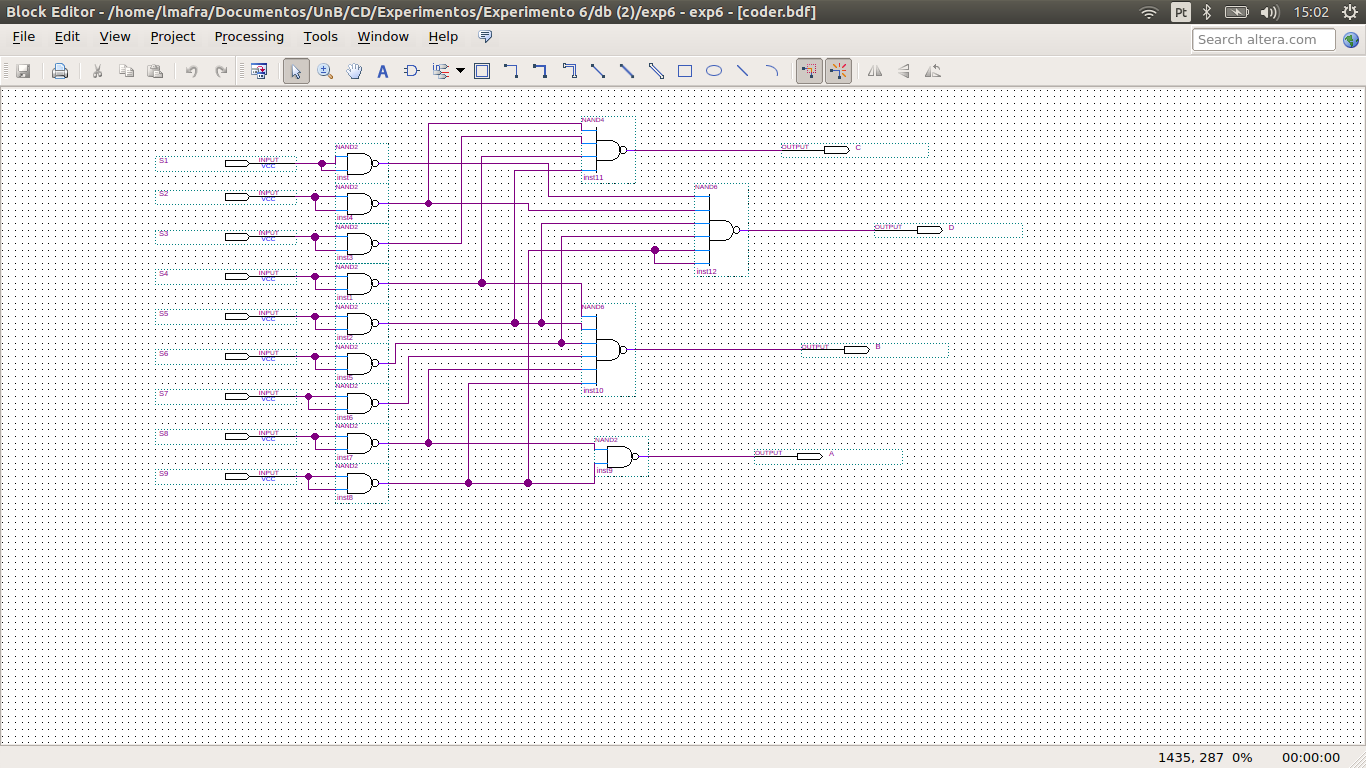
\includegraphics[width=1\textwidth]{coder.png}
	\caption{Diagrama Lógico do codificador.}
	\label{fig:coder}
\end{figure}

A partir do diagrama lógico total, realizamos a simulação funcional e temporal e obtivemos os seguintes gráficos.

\begin{figure}[H]
	\centering
	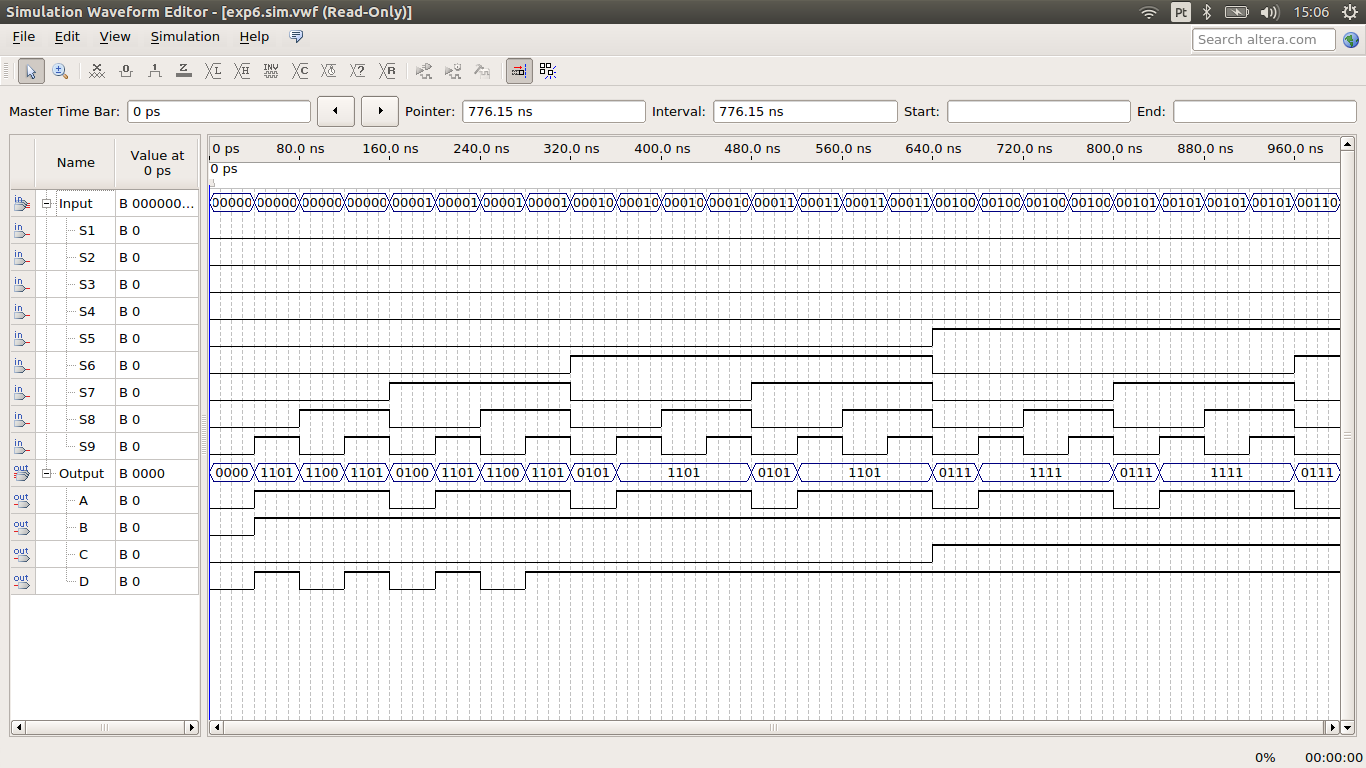
\includegraphics[width=1\textwidth]{functionalcoder.png}
	\caption{Simulação funcional do codificador.}
	\label{fig:funccoder}
\end{figure}

\begin{figure}[H]
	\centering
	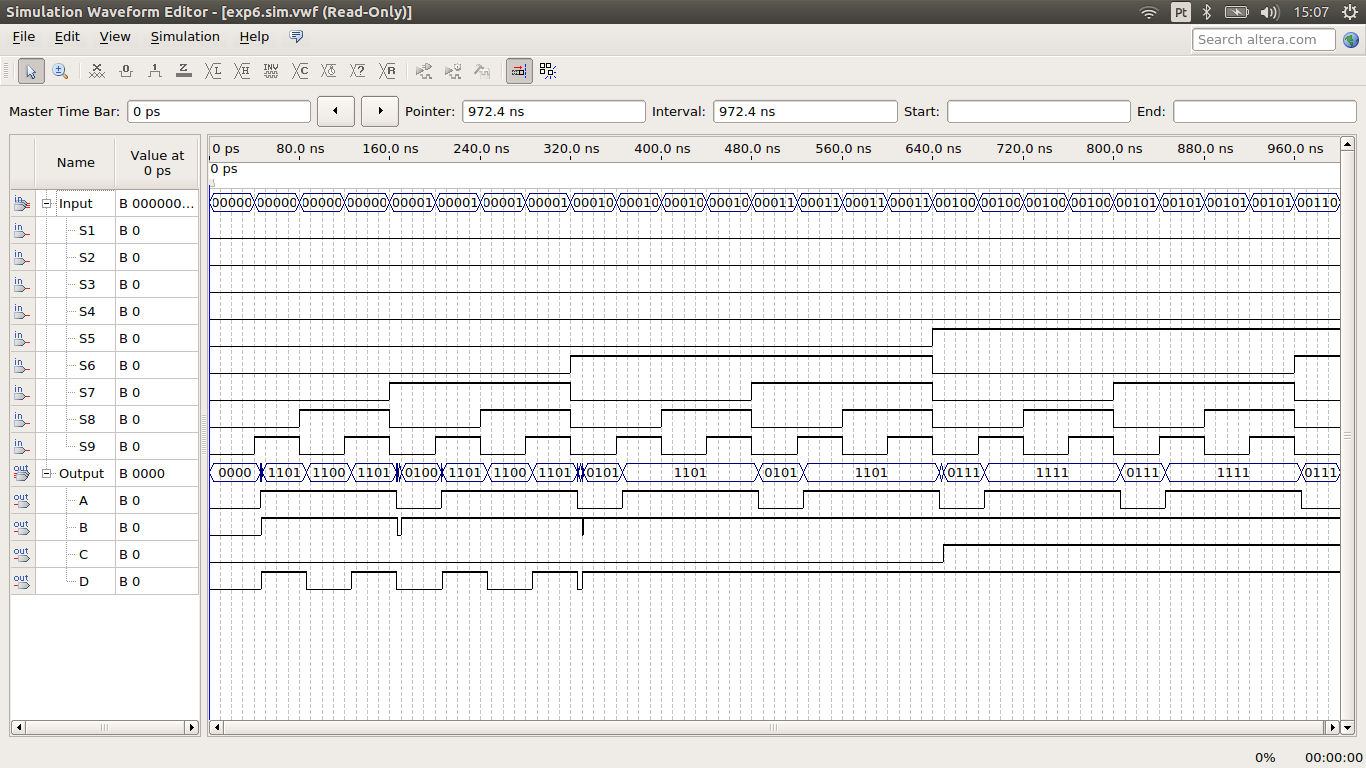
\includegraphics[width=1\textwidth]{timingcoder.png}
	\caption{Simulação temporal do codificador.}
	\label{fig:timecoder}
\end{figure}


\subsection{Funções Booleanas para o Decodificador}
\label{sec:Decod}

\begin{figure}[H]
	\centering
	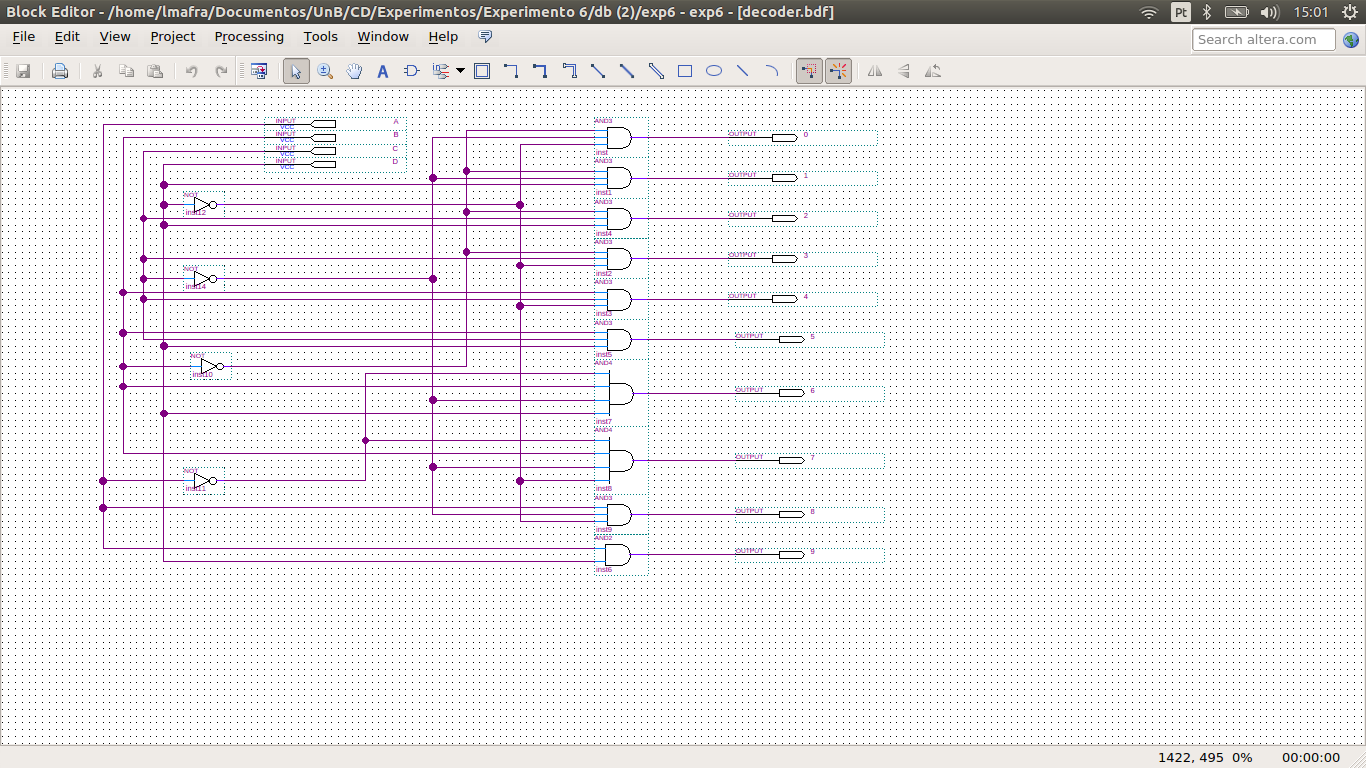
\includegraphics[width=1\textwidth]{decoder.png}
	\caption{Diagrama Lógico do decodificador.}
	\label{fig:decoder}
\end{figure}

\begin{figure}[H]
	\centering
	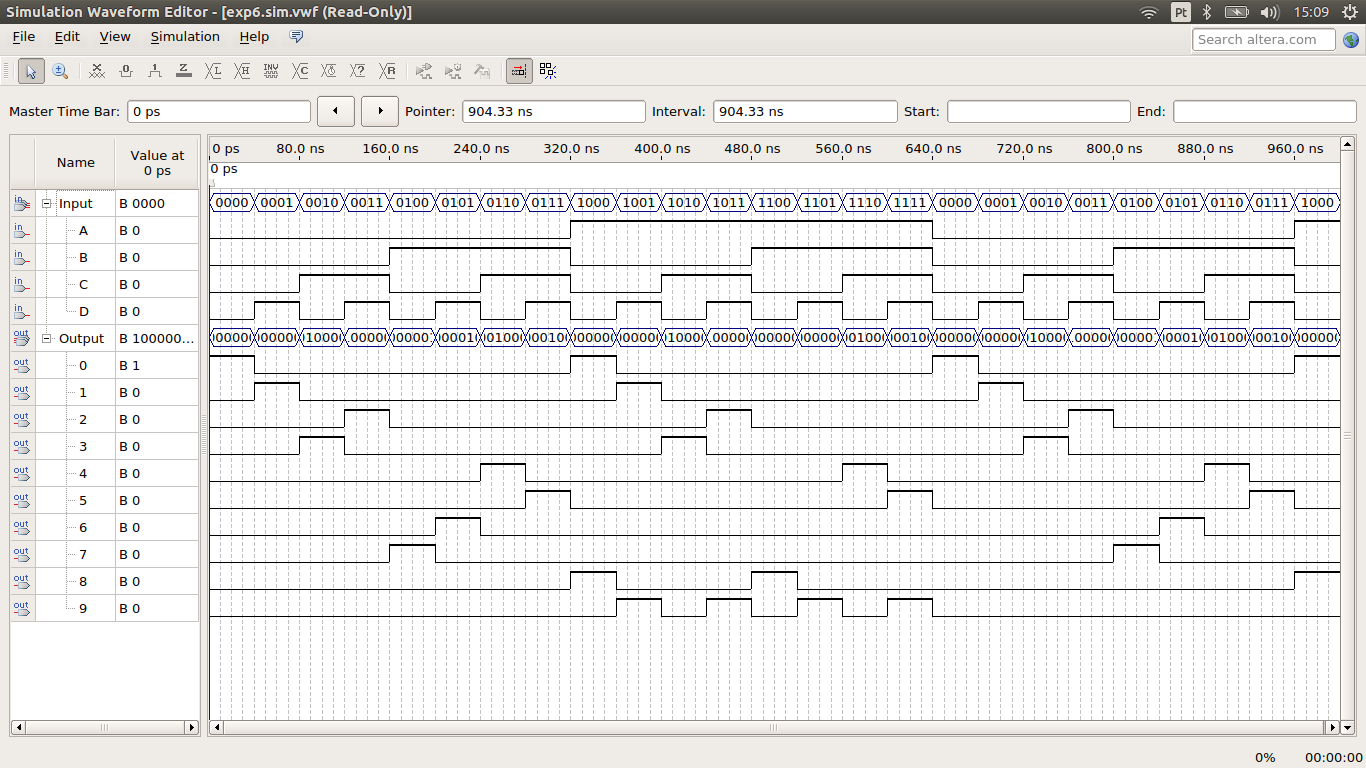
\includegraphics[width=1\textwidth]{functionaldecoder.png}
	\caption{Simulação funcional do decodificador.}
	\label{fig:funcdecoder}
\end{figure}

\begin{figure}[H]
	\centering
	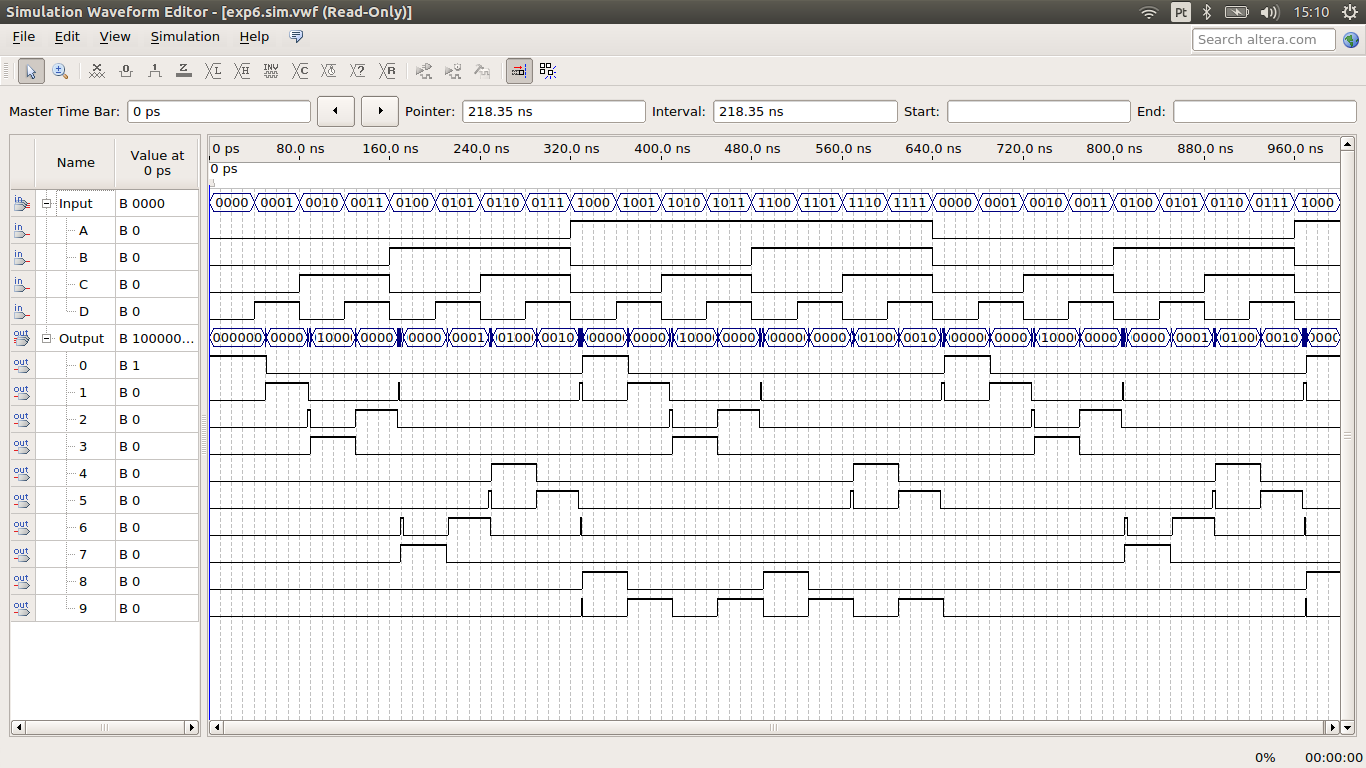
\includegraphics[width=1\textwidth]{timingdecoder.png}
	\caption{Simulação temporal do decodificador.}
	\label{fig:timedecoder}
\end{figure}

A tabela verdade abaixo 

\begin{table}[H]
	\centering
	\begin{tabular}{|c|c|c|c|c|}
		\cline{1-5}
		\multicolumn{1}{|c|}{Decimal} & \multicolumn{1}{|c|}{A} & \multicolumn{1}{|c|}{B} & \multicolumn{1}{|c|}{C} & \multicolumn{1}{|c|}{D}\\
		\hline
		S0 & 0 & 0 & 0 & 0 \\
		\hline
		S1 & 0 & 0 & 0 & 1 \\
		\hline
		S2 & 0 & 0 & 1 & 1 \\
		\hline
		S3 & 0 & 0 & 1 & 0 \\
		\hline
		S4 & 0 & 1 & 1 & 0 \\
		\hline
		S5 & 0 & 1 & 1 & 1 \\
		\hline
		S6 & 0 & 1 & 0 & 1 \\
		\hline
		S7 & 0 & 1 & 0 & 0 \\
		\hline
		S8 & 1 & 1 & 0 & 0 \\
		\hline
		S9 & 1 & 1 & 0 & 1 \\
		\hline
	\end{tabular}
	
\end{table} 




\subsection{Funcionamento do Codificador e Decodificador}

Desenvolvemos no kit de desenvolvimento em FPGA DE2 Altera o código projetado com o codificador e decodificador projetado na imagem abaixo. 

\begin{figure}[H]
	\centering
	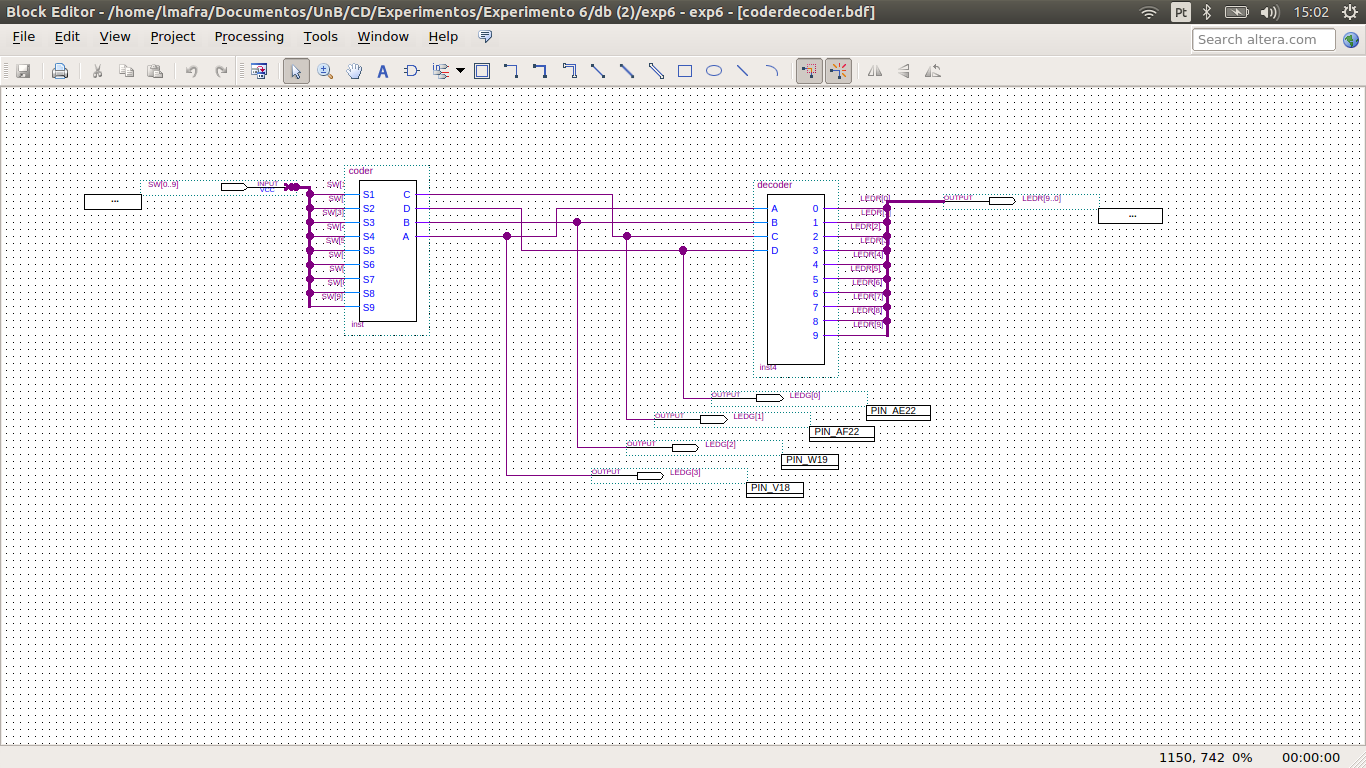
\includegraphics[width=1\textwidth]{coderdecoder.png}
	\caption{Circuito contendo codificador e decodificador.}
	\label{fig:coderdecoder}
\end{figure}

É possível ver o resultado no seguinte link: \href{https://www.youtube.com/watch?v=paRaiHqDqBo}{Vídeo no Youtube}


\section{Análise dos Resultados}
\label{sec:Resultados}

No experimento, tudo ocorreu como o esperado: a tabela verdade obtida a partir do diagrama de ondas estava de acordo com o que se queria que ambos circuitos fizessem, fato averiguado na placa Altera. Para todos os valores decimais de entrada, os LED’s verdes acenderam de forma correspondente aos seus código de Gray.
Sendo assim, obtivemos os resultados previstos na parte teórica, que foi obter os mapas de karnaugh do codificador e do decodificador, e o experimento foi um sucesso. 

\section{Conclusão}
\label{sec:Conclusao}

A partir do experimento foi possível ampliar os conhecimentos sobre codificadores e decodificadores. A montagem desses circuitos aperfeiçoou ainda mais a já conhecida teoria a respeito deles. Circuitos simples como esses são bases para o avanço da tecnologia, e de toda essa gama de aparelhos que temos hoje, eles abrem portas para muitas possibilidades e a familiarização com eles é, naturalmente, muito importante.


\bibliographystyle{sbc}
\bibliography{relatorio}


\newpage 
% Colocar aqui apenas as respostas dos itens da Auto-Avaliação
\section*{Auto-Avaliação}

\begin{enumerate}
    \item a
    \item c
    \item b
    \item c
    \item d
    \item Porta NOT A defeituosa, sempre com nível 0 na saída.
    \item Porta NOT D defeituosa, sempre com nível 1 na saída. 
    \item Porta NOT A defeituosa, sempre com nível 1 na saída.
\end{enumerate}


\end{document}
